\documentclass[
    aspectratio=169
]{beamer}
\usetheme{uob}

\usepackage{siunitx}
\usepackage{tikz}

\title{Monmouth STEM Presentation}

\date{15th October 2025}
\author{Christopher Davis}

\begin{document}

\begin{frame}
\titlepage
\end{frame}

\section{Introduction}

\begin{frame}{About me}
	\begin{columns}[T] % Align columns at the top
		% Left Column: Text
		\begin{column}{0.5\textwidth}
			\begin{itemize}
				\item Christopher Davis
				\item STEM Ambassador
				\item Railway Systems Engineer
				\item PhD Student at the University of Birmingham
				\item 
				\item Member:
				\item Institution of Engineering and Technology (IET)
				\item Institution of Railway Signal Engineers (IRSE)
				\item Institute for Systems Engineering (IfSE)
				
			\end{itemize}
		\end{column}
		
		% Right Column: Image
		\begin{column}{0.5\textwidth}
			\includegraphics[width=\textwidth]{images/headshot.jpeg}
		\end{column}
	\end{columns}
	
\end{frame}

\begin{frame}{History}
	\begin{columns}[T] % Align columns at the top
		% Left Column: Text
		\begin{column}{0.5\textwidth}
			\begin{itemize}
				\item Bishop's Stortford: School
				\item Bristol: Electrical and Electronic Engineering MEng
				\item Bristol: Internal Software Developer
				\item London: Arup, Railway Systems Engineer
				\item Birmingham: PhD Student
				
			\end{itemize}
		\end{column}
		
		% Right Column: Image
		\begin{column}{0.5\textwidth}
			\begin{tikzpicture}
				%Map
				\node[anchor=south west,inner sep=0] at (0,0) {\includegraphics[width=\textwidth]{images/uk_map.png}};
				%Leeds
				\draw[blue,ultra thick,rounded corners] (3.8,4.7) rectangle ++(0.4,0.3);
				%Stortford
				\draw[purple,ultra thick,rounded corners] (5,2.5) rectangle ++(0.3,0.3);
				%London
				\draw[black,ultra thick,rounded corners] (4.7,2) rectangle ++(0.5,0.4);
				%Bristol
				\draw[magenta,ultra thick,rounded corners] (3.1,1.95) rectangle ++(0.4,0.4);
				%Birmingham
				\draw[red,ultra thick,rounded corners] (3.4,3.1) rectangle ++(0.7,0.4);
			\end{tikzpicture}
		\end{column}
	\end{columns}
	\footnotetext[1]{Image Source; OpenStreetMap.org}
\end{frame}

\begin{frame}{Outside of Work}
	\begin{tikzpicture}
		%Cosmiques
		\node[anchor=south west,inner sep=0] at (0,0) {\includegraphics[width=5cm]{images/climbing1.jpg}};
		
		%Scotland
		\node[anchor=south west,inner sep=0] at (4.5,0) {\includegraphics[width=5cm]{images/climbing3.jpg}};
		
		%Lundy
		\node[anchor=south west,inner sep=0] at (9,3) {\includegraphics[width=3.5cm]{images/climbing5.jpg}};
		
		%Cornwall
		\node[anchor=south west,inner sep=0] at (11,0) {\includegraphics[width=3.5cm]{images/climbing4.jpg}};
		
		%YRP
		\node[anchor=south west,inner sep=0] at (4.8,3.7) {\includegraphics[width=4.3cm]{images/yrp1.jpg}};
		
		
	\end{tikzpicture}
	
\end{frame}

\section{Railway Engineering}

\begin{frame}{What is Engineering?}
\end{frame}

\begin{frame}{Engineering Definitions}
	\begin{exampleblock}{Engineering Council}
		``Chartered Engineers (CEng) develop solutions to engineering problems using new or existing technologies, through innovation, creativity and change``
	\end{exampleblock}
	\begin{exampleblock}{Wikipedia}
		``Engineering is the practice of using natural science, mathematics, and the engineering design process to solve problems within technology, increase efficiency and productivity, and improve systems.``
	\end{exampleblock}
	\begin{exampleblock}{NASA}
		``Engineers solve problems.``
	\end{exampleblock}
\end{frame}

\begin{frame}{What is Railway Engineering?}
	
\end{frame}

\begin{frame}{Railway Engineering Disciplines}
	\begin{columns}[T] % Align columns at the top
		% Left Column: Text
		\begin{column}{0.5\textwidth}
			\begin{itemize}
				\item Rolling Stock (Trains) (Mechanical / Electrical)
				\item Permanent Way (Track) (Mechanical / Civil)
				\item Bridges (Structural Engineers)
				\item Tunnels (Civil / Geotechnical Engineers)
				\item Stations (Structural Engineers)
				\item Signalling (Electrical)
				\item Timetabling / Transport Planning (Geography)
			\end{itemize}
		\end{column}
		
		% Right Column: Image
		\begin{column}{0.5\textwidth}
			\includegraphics[width=\textwidth]{images/station.jpg}
		\end{column}
	\end{columns}
	\footnotetext[1]{Image Source: TheFrog001, Wikimedia Commons}
	
\end{frame}

\begin{frame}{Different Views of a System}
	\begin{itemize}
		\item Tube map
		\item Carto Metro
		\item undergrounddistances
	\end{itemize}
\end{frame}

\begin{frame}{My Research}
	\begin{columns}[T] % Align columns at the top
		% Left Column: Text
		\begin{column}{0.5\textwidth}
			\begin{itemize}
				\item Research into modelling and simulation of novel transport operating concepts
				\item Design a language to describe system architectures that is understandable by both humans and computers
			\end{itemize}
		\end{column}
		
		% Right Column: Image
		\begin{column}{0.5\textwidth}
			\includegraphics[width=\textwidth]{images/service-all-stop.png}
			\includegraphics[width=\textwidth]{images/service-express-local.png}
			\includegraphics[width=\textwidth]{images/service-dss.png}
		\end{column}
	\end{columns}
	
\end{frame}

\section{Activity}

\begin{frame}{Activity: Introduction}
	\begin{itemize}
		\item Railway networks rely on precise scheduling to ensure trains run safely, efficiently and on time
		\item A train graph is a type of time-distance diagram used to visualise how train move through a network
		\item It helps planners
		\begin{itemize}
			\item Check for conflicts between services
			\item Spot delays or inefficiencies
			\item Ensure trains maintain safe spacing and arrive on time
		\end{itemize}
		\item In this activity you'll take the role of a timetable planner
		\item Your goal is to design a conflict free schedule using a train graph
	\end{itemize}
\end{frame}

\begin{frame}{Activity: Example Train Graph}
	\includegraphics[width=\textwidth]{../train-generator/output/victoria.png}
\end{frame}

\begin{frame}{Activity: Your Task}
	\begin{center}
		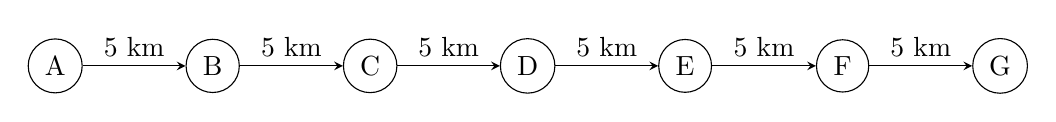
\begin{tikzpicture}[->, >=stealth, node distance=2cm]
			\node[circle, draw] (a) {A};
			\node[circle, draw, right of=a] (b) {B};
			\node[circle, draw, right of=b] (c) {C};
			\node[circle, draw, right of=c] (d) {D};
			\node[circle, draw, right of=d] (e) {E};
			\node[circle, draw, right of=e] (f) {F};
			\node[circle, draw, right of=f] (g) {G};
			
			\draw (a) -- (b) node[midway, above] {5 km};
			\draw (b) -- (c) node[midway, above] {5 km};
			\draw (c) -- (d) node[midway, above] {5 km};
			\draw (d) -- (e) node[midway, above] {5 km};
			\draw (e) -- (f) node[midway, above] {5 km};
			\draw (f) -- (g) node[midway, above] {5 km};
		\end{tikzpicture}
	\end{center}
	
	\begin{itemize}
		\item All service must depart within \qty{60}{\minute}
		\item The schedule must be designed so that it can be repeated every hour without conflicts.
		\item A minimum Headway of \qty{5}{\minute} must be maintained between any two trains at any point along the line.
		\item Dwell time must be applied at each scheduled stop.
	\end{itemize}
	\begin{center}
		\begin{tabular}{@{}lllll@{}}
			\toprule
			Train Type & TPH & Max Velocity (\unit{\km \per \hour}) & Stops & Dwell (\unit{\minute}) \\ \midrule
			Express      & 2                 & 120      & D                  & 2.5                   \\
			Local    & 2                 & 80       & All                & 7                     \\
			Freight    & 1                 & 60       & None               &                       \\ \bottomrule
		\end{tabular}
	\end{center}
	
\end{frame}

\section{Discussion}

\begin{frame}{Activity: Discussion}
	
\end{frame}

\begin{frame}{Activity: My Train Graph - Standard}
	\includegraphics[width=\textwidth]{../train-generator/output/activity-even.png}
\end{frame}

\begin{frame}{Activity: My Train Graph - Extra Local}
	\includegraphics[width=\textwidth]{../train-generator/output/activity-even-extra.png}
\end{frame}

\begin{frame}{Activity: My Train Graph - Grouped}
	\includegraphics[width=\textwidth]{../train-generator/output/activity-grouped.png}
\end{frame}

\section{Questions}

\begin{frame}{Questions}
	
\end{frame}

\end{document}